\chapter{Tổng quan tình hình nghiên cứu}
% Sơ lược, phân tích, đánh giá các công trình nghiên cứu nổi tiếng có liên quan đến đề tài. Nêu những vấn đề bức thiết cần phải giải quyết, chỉ ra những thiếu sót mà những nghiên cứu trước đây chưa giải quyết được.

\section{Bài nghiên cứu "Lip Movements Generation at a Glance"\cite{chen2018}}

\begin{figure}[H]
    \centering
    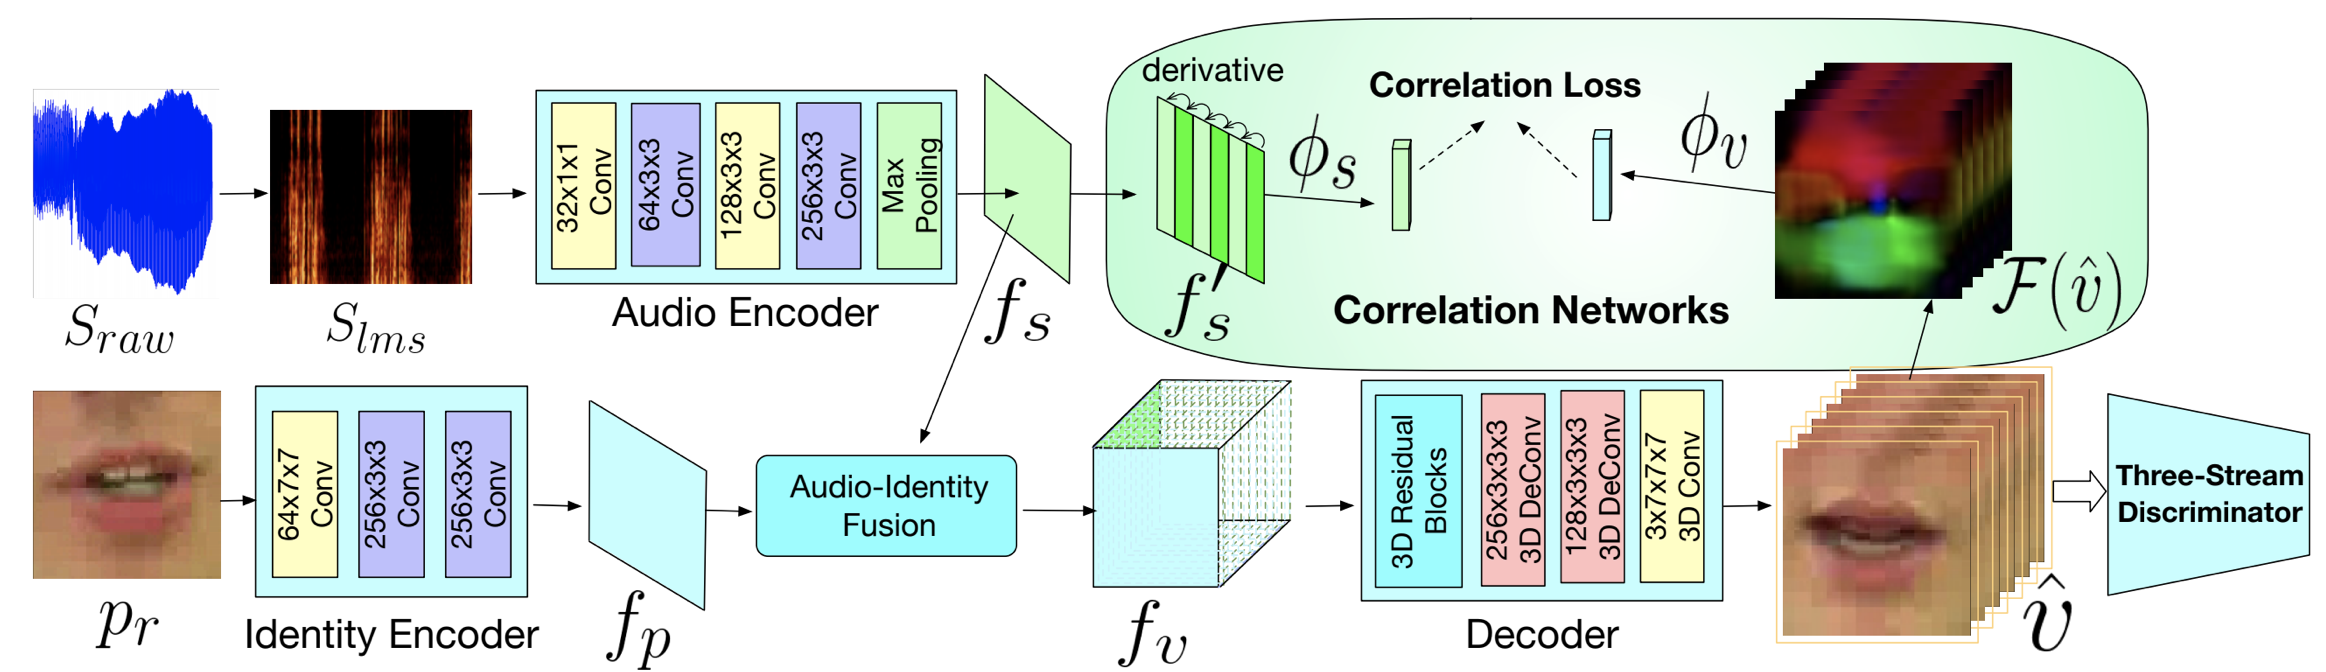
\includegraphics[width=15cm]{./content/images/chen2018_model.png}
    \caption{Mô hình của bài báo Lip Movements Generation at a Glance}
    \label{fig:chen2018_model}
\end{figure}

Việc tạo sinh khẩu hình miệng khớp với tiếng nói là bước đầu tiên để thực hiện việc tạo sinh khuôn mặt. Nghiên cứu này đã thành công trong việc tạo sinh khẩu hình miệng từ một ảnh tĩnh chứa hình ảnh khuôn miệng của một người bất kỳ, và một đoạn âm thanh chứa tiếng nói. Bằng phương pháp kết hợp các đặc trưng âm thanh và hình ảnh, nghiên cứu cho ra kết quả tốt và có độ chính xác cao hơn so với các nghiên cứu trước đó. Hình \ref{fig:chen2018_model} mô tả cấu trúc của mạng tạo sinh ảnh được dùng. Đầu tiên, âm thanh được cắt thành các đoạn nhỏ dài 0.64s, các đoạn này được chuyển thành phổ Log-Mel ($S_{raw}$ thành $S_{lms}$), sau đó qua một bộ Audio Encoder để trích đặc trưng, ta có đặc trưng âm thanh $f_s$ là một ma trận 2 chiều kích thước $F \times T$. Bên cạnh đó, hình ảnh khuôn miệng cũng được đưa qua một bộ Identity Encoder để tạo thành ma trận 2 chiều $f_p$ kích thước $H \times W$.

\begin{figure}[H]
    \centering
    \begin{minipage}{0.48\textwidth}
        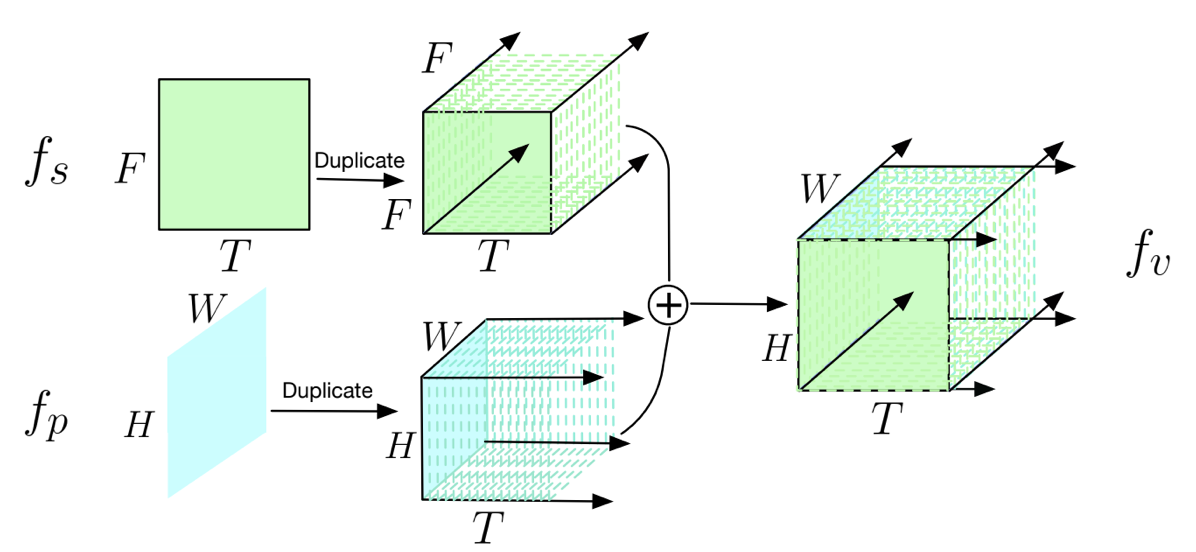
\includegraphics[width=7cm]{./content/images/chen2018_fusion.png}
        \caption{Phương pháp kết hợp đặc trưng hình ảnh và âm thanh}
        \label{fig:chen2018_fusion}
    \end{minipage}\hfill
    \begin{minipage}{0.48\textwidth}
        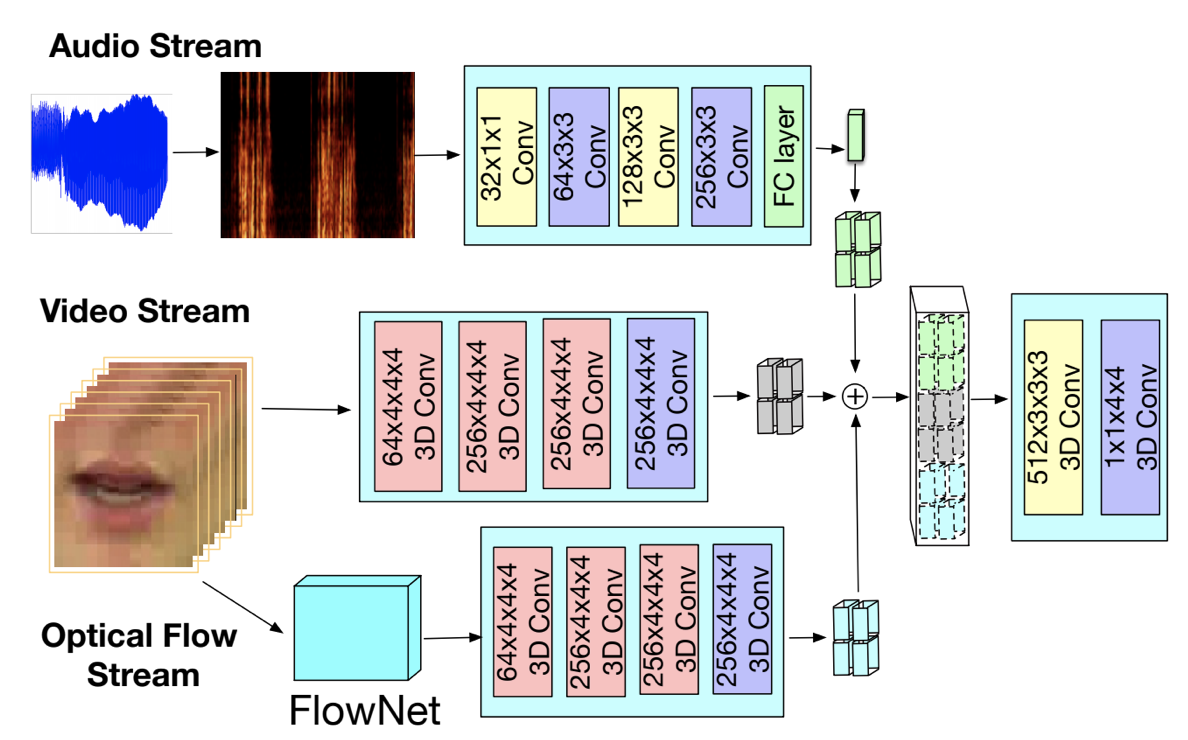
\includegraphics[width=7cm]{./content/images/chen2018_gans.png}
        \caption{GANs Discriminator với 3 loại đặc trưng}
        \label{fig:chen2018_gans}
    \end{minipage}
\end{figure}

Để kết hợp hai đặc trưng hình ảnh, âm thanh với nhau để tạo sinh hình ảnh mới, tác giả bài báo đề xuất phương pháp nhân bản ma trận $f_s$ F lần và nhân bản ma trận $f_p$ T lần thành hai tensor ba chiều, sau đó nối tiếp các kênh của hai tensor này để tạo thành khối tensor ba chiều mới. Để có thể nối tiếp được với nhau, Tác giả đã đặt các thông số $H = W = F$. Hình \ref{fig:chen2018_fusion} miêu tả cách kết hợp hai đặc trưng hình ảnh - âm thanh thành khối đặc trưng chung $f_v$, khối $f_v$ có kích thước $W \times H \times T$. Khối đặc trưng này sau cùng được chuyển đổi thành ảnh đầu ra $\hat{v}$ nhờ vào mạng Decoder. Mạng Decoder này sử dụng kiến trúc 3D Residual và các khối Deconvolution nhằm bảo toàn các đặc điểm của hình ảnh gốc.

Đồng thời, nghiên cứu này cũng chỉ ra rằng đặc tính của khuôn miệng trong video là hình ảnh thường đi trước âm thanh, và độ trễ âm thanh - hình ảnh là không đồng nhất trong các video khác nhau. Vì vậy, để tạo sinh một video chân thực, ta phải quan tâm đến độ trễ này. Khối Correlation Network trong hình \ref{fig:chen2018_model} miêu tả cách tính toán giá trị Corelation Loss. Để tính giá trị này, bộ tính toán cần có một encoder ($\phi_s$) để encode sự thay đổi của âm thanh và một encoder ($\phi_v$) để encode sự thay đổi của hình ảnh. Ma trận $f_s$ được tính đạo hàm theo trục T thành $f'_s$, hình ảnh được tạo sinh $\hat{v}$ cũng được đưa qua hàm $\mathcal{F}$ để lấy đặc trưng Optical Flow. Sau đó, cả hai đặc trưng thể hiện sự thay đổi của âm thanh và hình ảnh theo thời gian này được đưa qua các encoder $\phi_s$ và $\phi_v$ để tạo ra hai vector có cùng số chiều. Công thức tính của giá trị Correlation Loss chính là hiệu của 1 và giá trị cosin giữa hai vector đặc trưng cuối cùng:

\begin{equation}
    \ell_{corr} = 1 - \frac{\phi_s(f'_s)\cdot\phi_v(\mathcal{F}(v))}{\|\phi_s(f'_s)\|_2\cdot\|\phi_v(\mathcal{F}(v))\|_2}
    \label{eqn:chen2018_corr_loss}
\end{equation}


Cấu trúc mạng GANs cũng đã được sử dụng trong nghiên cứu này nhằm mục đích tạo ra chuyển động mượt mà cho chuỗi hình ảnh trong video và làm cho chất lượng ảnh tạo sinh tốt hơn. Bộ phân biệt (Discriminator) giữa ảnh thật và ảnh tạo sinh ($D$) được miêu tả trong hình \ref{fig:chen2018_gans}. Đặc trưng Log-Mel của âm thanh được encode thành một vector bằng một mạng Convolution - Fully connected, sau đó vector này được nhân bản và ghép nối để có số chiều bằng với tensor của hai đặc trưng còn lại. Hình ảnh được đưa vào mạng được encode bởi các khối 3D Convolution để có được tensor đặc trưng ảnh. Các ảnh này cũng được đưa qua mạng FlowNet để đưa ra đặc trưng Optical Flow, đặc trưng này cũng được encode để tạo ra tensor đặc trưng cho chuyển động trong video. Sau cùng, ba đặc trưng này được ghép nối tiếp theo kênh và được đưa qua các khối 3D Convolution để lấy được xác suất dự đoán ảnh thật hay tạo sinh của mạng. Cặp video - âm thanh đưa vào mạng có thể là video thật và đoạn âm thanh khớp với video đó, hoặc video thật và một đoạn âm thanh khác, hoặc video được tạo sinh và đoạn âm thanh tương ứng tạo ra nó. Hàm mất mát của mạng được định nghĩa như sau:

\begin{equation}
    \ell_{dis} = -logD([s^j, v^j]) - \lambda_plog(1 - D([s^j, \hat{v}])) - \lambda_ulog(1 - D([s^j, v^k])), k \ne j
\end{equation}

Để so sánh sự tương đồng về mặt tổng quan giữa hai video (video thật và video được tạo sinh), tác giả sử dụng một bộ Autoencoder. Bộ Autoencoder này được huấn luyện độc lập với mạng chính và sử dụng cùng bộ dữ liệu với mạng chính. Phần encoder ($\varphi$) được giữ lại để encode hình ảnh từ video nhằm mục đích trích xuất đặc trưng của chuỗi hình ảnh. Hàm Perceptual Loss $\ell_{perc}(\hat{v}, v)$ được dùng để tính toán độ sai lệch về mặt tổng quan giữa video được tạo sinh từ tiếng nói và video thật tương ứng với tiếng nói:
\begin{equation}
    \ell_{perc}(\hat{v}, v) = \|\varphi(v) - \varphi(\hat{v})\|^2_2
    \label{eqn:chen2018_perc_loss}
\end{equation}

Hàm mất mát của cuối cùng của mạng được định nghĩa:
\begin{equation}
    \mathcal{L} = \ell_{corr} + \lambda_1\ell_{pix} + \lambda_2\ell_{perc} + \lambda_3\ell_{gen}
    \label{eqn:chen2018_loss}
\end{equation}

Trong đó:
\begin{itemize}
\item $\ell_{corr}$: Là giá trị mất mát do sự sai lệch giữa hình ảnh và âm thanh đã nêu ở (\ref{eqn:chen2018_corr_loss}).
\item $\ell_{pix}$: Giá trị mất mát dựa trên sự sai khác ở cấp độ điểm ảnh giữa ảnh được tạo sinh và ảnh trong video thật, $\ell_{pix} = \|v-\hat{v}\|$.
\item $\ell_{perc}$: Giá trị mất mát đo độ sai khác trên toàn bộ chuỗi hình ảnh (đã nêu ở (\ref{eqn:chen2018_perc_loss})).
\item $\ell_{gen}$: Giá trị mất mát của bộ tạo sinh ảnh dựa trên hàm phân biệt $D$: $\ell_{gen} = -logD([s^j, \hat{v}^j])$.
\end{itemize}

Mô hình được huấn luyện và kiểm thử trên các tập dữ liệu GRID, LDC và LRW. Kết quả kiểm thử cho thấy mô hình này cho kết quả tạo sinh hình ảnh tốt hơn hẳn so với các nghiên cứu trước đó. Các độ đo PSNR, SSIM, LMD và CPBD được sử dụng để kiểm chứng. Sau đây là kết quả được khảo sát bới tác giả:

\begin{figure}[H]
    \centering
    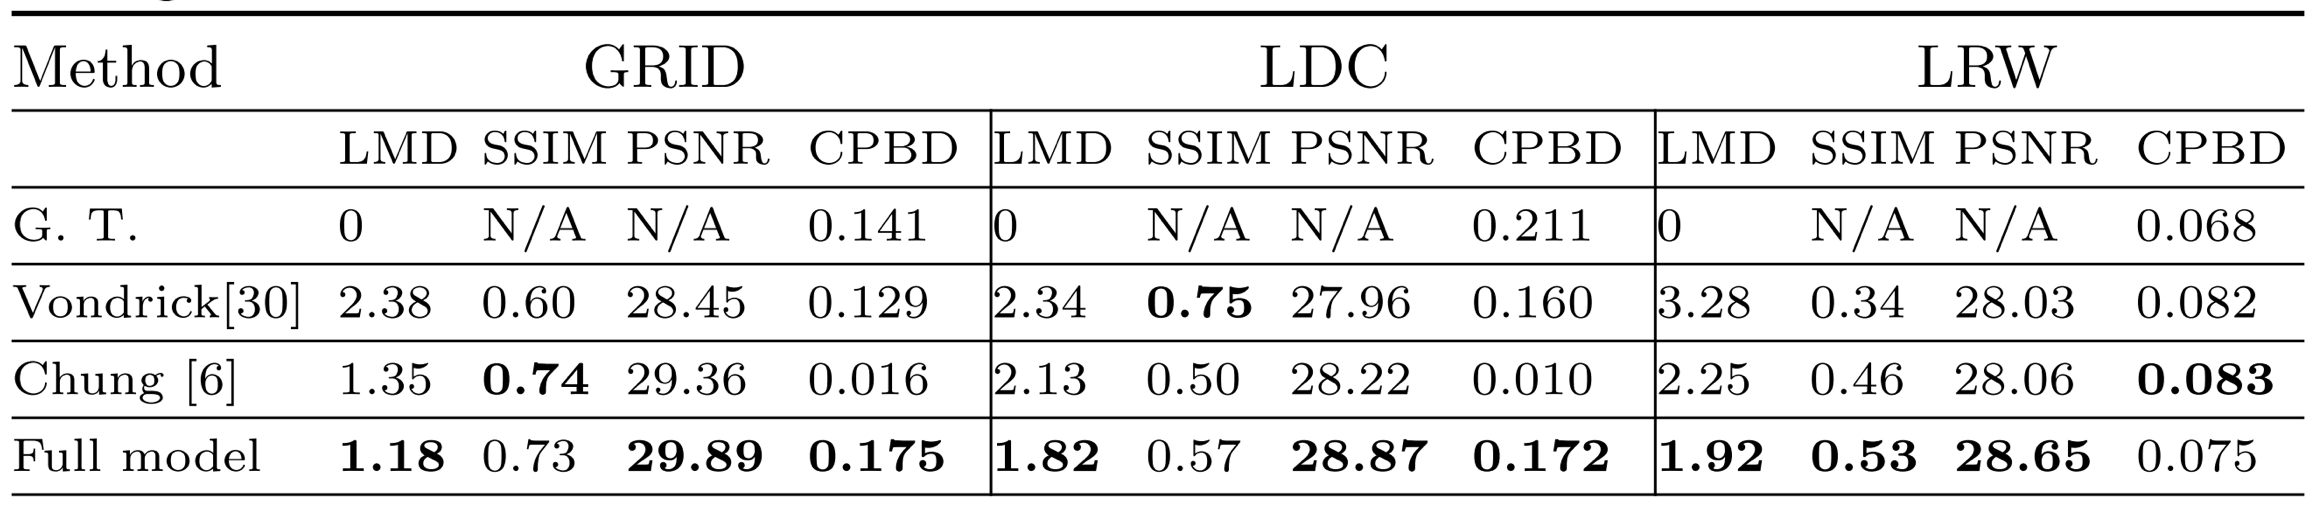
\includegraphics[width=15cm]{./content/images/chen2018_result.png}
    \caption{Kết quả đánh giá và so sánh mô hình trong nghiên cứu Lip Movements Generation at a Glance}
    \label{fig:chen2018_result}
\end{figure}

Nghiên cứu này đã đưa ra các phương pháp phù hợp và tiến bộ để trích xuất và kết hợp đặc trưng hình ảnh và âm thanh, đồng thời cũng tận dụng phương pháp GANs để cải thiện chất lượng của ảnh được tạo sinh. Độ hiệu quả của cấu trúc mạng được thể hiện qua kết quả đo lường vượt trội so với các nghiên cứu cùng thời điểm. Tuy nhiên, cấu trúc mạng này có một số yếu điểm. Thứ nhất, mạng chỉ có thể nhận vào hình ảnh tĩnh và một đoạn âm thanh có độ dài xác định (0.64s) và cho ra số khung hình tương ứng với khoảng thời gian đó (16 khung hình). Thứ hai, tác giả vẫn chưa chú ý đến hiện tượng nhảy hình của video được tạo sinh, mạng không có cơ chế để đảm bảo việc chuyển ảnh mượt mà, ít sai khác về độ tương phản, ánh sáng, màu sắc giữa các khung ảnh gần nhau.

%------------------------------------------------------------------------

\section{Bài nghiên cứu "End-to-End Speech-Driven Facial Animation with Temporal GANs"\cite{vougioukas2019}}
\label{sec:vougioukas2019}

\begin{figure}[H]
    \centering
    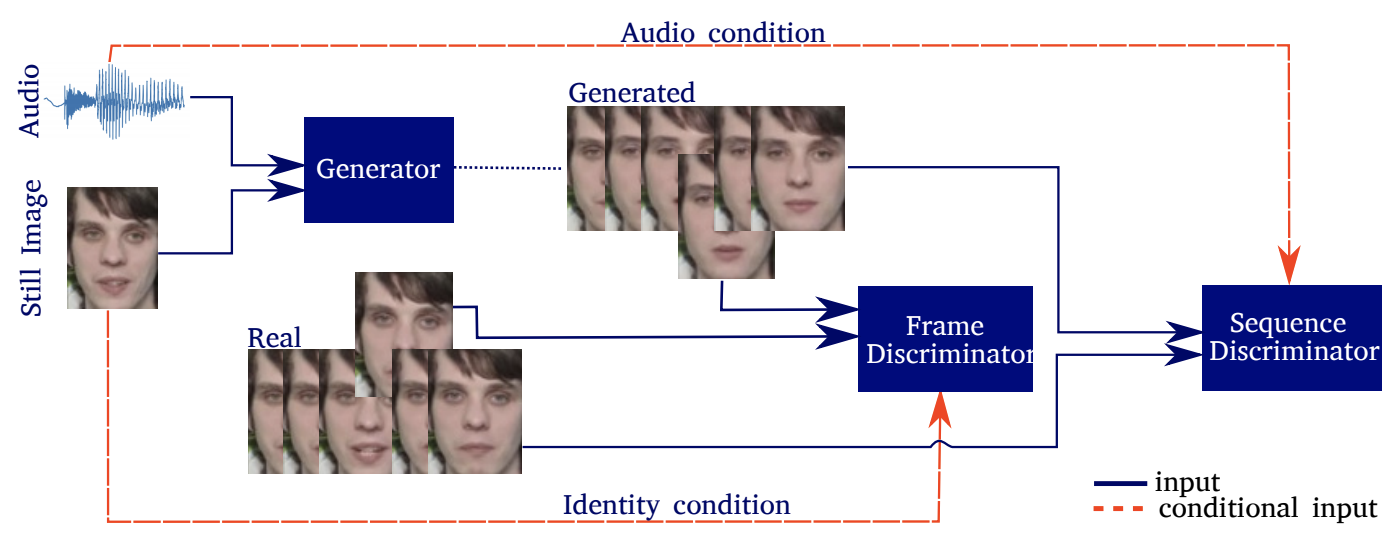
\includegraphics[width=15cm]{./content/images/vou2019_model.png}
    \caption{Mô hình của nghiên cứu End-to-End Speech-Driven Facial Animation with Temporal GANs}
    \label{fig:vou2019_model}
\end{figure}

Nghiên cứu của Vougioukas vào năm 2019 có mục tiêu là tạo ra chuỗi hình ảnh của toàn bộ gương mặt người đang nói với đầu vào là một ảnh tĩnh chứa mặt người bất kỳ và một đoạn tiếng nói bất kỳ. Kiến trúc của mạng được miêu tả trong hình \ref{fig:vou2019_model}, được bao gồm ba phần chính. Bộ tạo sinh ảnh Generator nhận vào một đoạn âm thanh tiếng nói có độ dài bất kỳ và một ảnh tĩnh, sử dụng những dữ liệu này như một gợi ý để tạo sinh chuỗi hình ảnh mới với mặt người đang nói tiếng nói tương ứng. Bộ phân biệt ảnh theo khung hình Frame Discriminator cũng nhận vào ảnh tĩnh nói trên, đồng thời nhận thêm một ảnh khác, ảnh này hoặc được tạo sinh từ Generator, hoặc được trích xuất từ video trong bộ dữ liệu. Frame Discriminator sẽ được huấn luyện để phân biệt đâu là ảnh được tạo sinh và đâu là ảnh thật được trích xuất từ video huấn luyện. Bộ phân biệt chuỗi ảnh Sequence Discriminator nhận vào đoạn tiếng nói và một chuỗi hình ảnh trong video. Chuỗi hình ảnh này có thể là hình ảnh được tạo sinh hoặc hình ảnh gốc từ video tương ứng. Bộ Sequence Discriminator sẽ học cách phân biệt hai loại video này trong quá trình huấn luyện. Theo như cơ chế GANs, trong quá trình huấn luyện, hàm mất mát của hai bộ Discriminator sẽ tạo ra lan truyền ngược và cập nhật trọng số của chính nó và của cả Generator. Từ đó, cả ba mạng này đều sẽ dần trở nên chính xác hơn.

\begin{figure}[H]
    \centering
    \begin{minipage}{0.48\textwidth}
        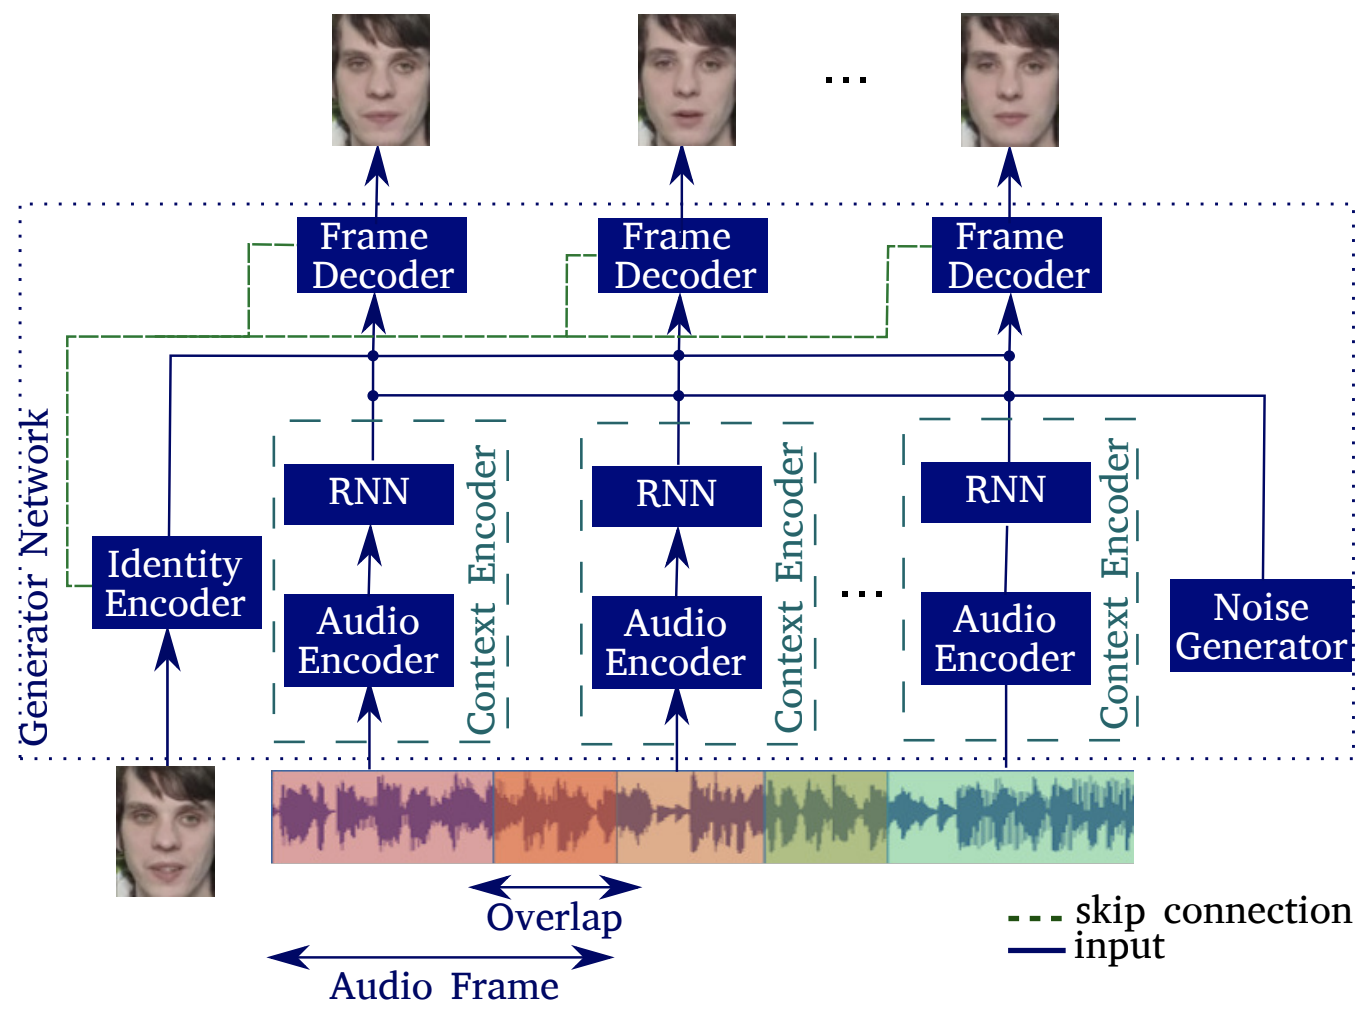
\includegraphics[width=7cm]{./content/images/vou2019_gen.png}
        \caption{Kiến trúc bộ Generator}
        \label{fig:vou2019_gen}
    \end{minipage}\hfill
    \begin{minipage}{0.48\textwidth}
        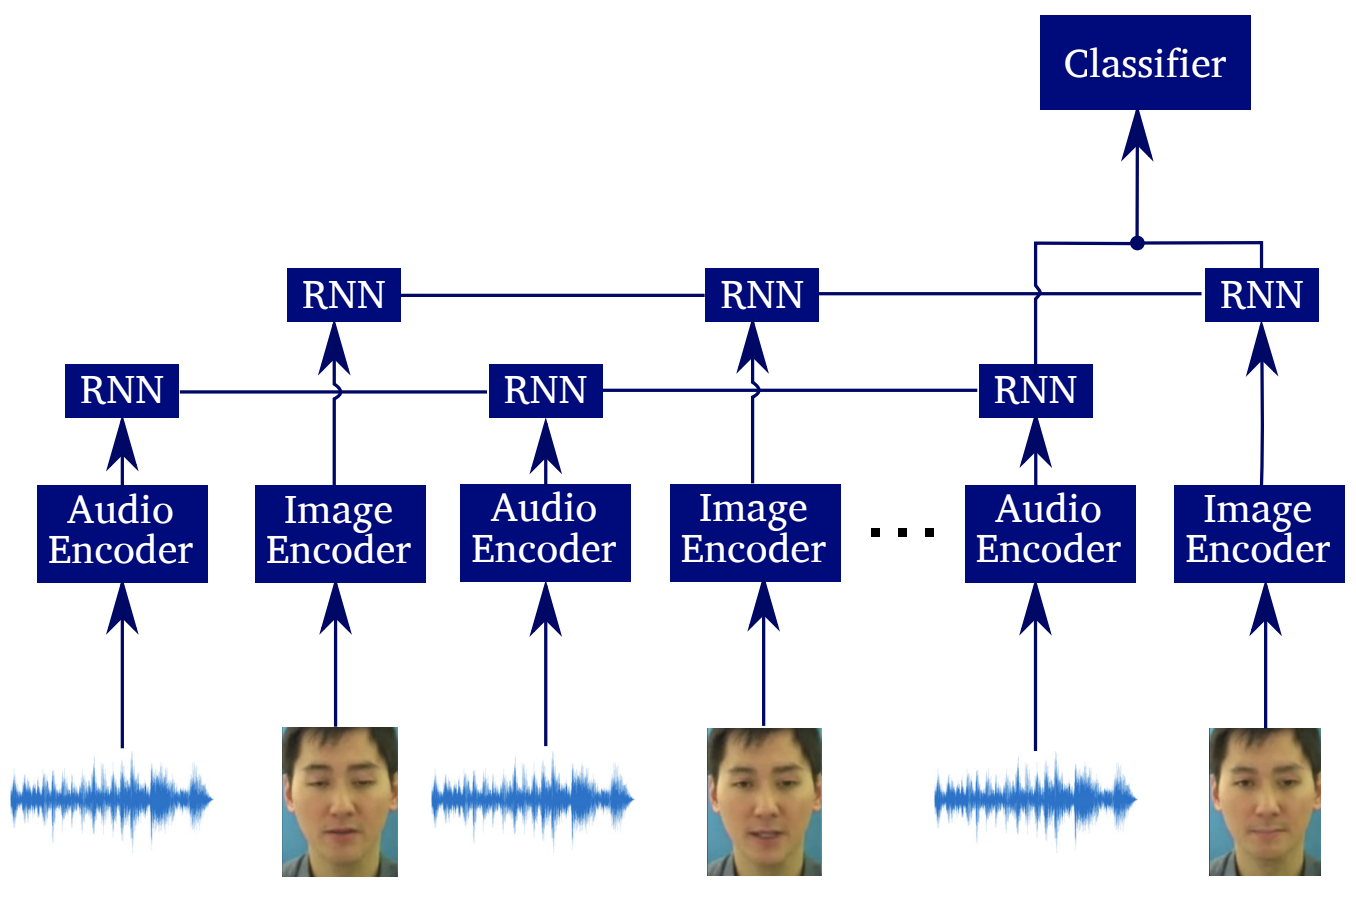
\includegraphics[width=7cm]{./content/images/vou2019_seq_dis.png}
        \caption{Kiến trúc bộ Sequence Discriminator}
        \label{fig:vou2019_seq_dis}
    \end{minipage}
\end{figure}

Trong nghiên cứu này, video huấn luyện được tách riêng thành âm thanh và hình ảnh. Mỗi khung hình kích thước $96\times128$ được cắt ra từ video tương ứng với đoạn âm thanh dài 0.16s, đoạn âm thanh này tạo thành một vector 8000 điểm. Như vậy, dữ liệu được tiền xử lý bằng cách cắt nhỏ video thành khung ảnh và đoạn âm thanh tương ứng với ảnh đó (âm thanh có chồng lấn giữa các ảnh).

Kiến trúc của bộ tạo sinh chuỗi ảnh Generator được miêu tả trong hình \ref{fig:vou2019_gen}. Identity Encoder là bộ encoder ảnh có tính năng trích xuất đặc trưng của ảnh tĩnh được đưa vào mạng. Bộ encoder này gồm 6 lớp 2D Convolution, mỗi lớp kết hợp với Batchnorm và ReLU ở phía sau. Mạng này giúp trích xuất ảnh đầu vào thành vector 50 chiều ($z_{id}$). Context Encoder là tổng hợp của hai bộ bao gồm Audio Encoder và một bộ RNN hai lớp. Audio Encoder sẽ trích xuất đặc trưng từ đoạn âm thanh 8000 điểm (vector 8000 chiều) để tạo ra vector 256 chiều. Đặc trưng này được đưa vào bộ RNN để bổ sung ngữ nghĩa về mặt thời gian. Ngõ ra của bộ Context Encoder là trạng thái ẩn (hidden state) của bộ RNN có số chiều bằng 256 ($z_c$). Generator còn có một bộ Noise Generator, thực chất là một mạng GRU có chức năng tạo ra vector nhiễu Gauss 10 chiều ($z_n$). $z_{id}$, $z_c$ và $z_n$ được ráp nối với nhau theo kênh tương ứng trước khi đưa vào bộ tạo sinh ảnh. Trong khi $z_{id}$ có chức năng giúp Frame Decoder tái tạo chính xác gương mặt của người nói, $z_c$ sẽ mang thông tin về mặt âm thanh, thời gian và hoàn cảnh, giúp tạo ra gợi ý cho mạng để tạo sinh được hình ảnh tương ứng với âm thanh. Đồng thời, $z_n$ tạo ra tính ngẫu nhiên cho mạng, khi đưa cùng một đầu vào, thì sẽ không khi nào mạng cho ra kết quả giống nhau ở hai lần thử. Đồng thời, tính ngẫu nhiên này lại có tính chất phụ thuộc thời gian (do được tạo ra bởi mạng GRU) đem lại cho hình ảnh được tạo sinh các biểu cảm nhỏ như nháy mắt và các chuyển động nhỏ trên mặt một cách liền lạc.

Ở đầu ra, bộ sinh ảnh Frame Decoder được sử dụng để tạo sinh chuỗi ảnh theo thời gian. Vector đặc trưng ẩn có 316 chiều, từ vector đặc trưng này, Frame Decoder sẽ tạo ra hình ảnh có kích thước bằng với hình mẫu ban đầu ($96\times128$). Nhằm bảo toàn nhận dạng của người trong ảnh mẫu, Frame Decoder được thiết kế theo kiến trúc U-Net gồm 6 lớp Convolution tương ứng với Identity Encoder. Các lớp Convolution này nhận thêm các đặc trưng ẩn từ lớp tương ứng của Identity Encoder để hạn chế việc đánh mất nhận dạng của mặt người mẫu do bị ảnh hưởng bởi độ sâu của mạng. Các đặc trưng ẩn đi qua các lớp Deconvolution và cuối cùng tạo ra ảnh tương ứng với âm thanh.

Bộ phân biệt khung ảnh Frame Discriminator trong hình \ref{fig:vou2019_model} là một mạng Convolution 6 lớp, đầu ra của mạng là xác suất ảnh này được cho là ảnh được tạo sinh. Frame Discriminator giúp cho ảnh tạo sinh từ Generator chân thực hơn, khó phân biệt với ảnh từ video gốc hơn. Bộ phân biệt chuỗi ảnh Sequence Discriminator được miêu tả trong hình \ref{fig:vou2019_seq_dis} có cấu trúc trích xuất đặc trưng tương tự như bộ Generator. Sự khác biệt đến từ bộ trích xuất đặc trưng chuỗi ảnh. Chuỗi hình ảnh được đưa qua bộ Image Encoder để trích xuất đặc trưng ảnh và thu nhỏ số chiều dữ liệu. Các ảnh sau khi qua bộ Image Encoder sẽ được đưa vào mạng RNN hai lớp để cập nhật trạng thái ẩn của mạng RNN. Khi kết thúc chuỗi hình ảnh và âm thanh tương ứng với nó, trạng thái ẩn của hai mạng RNN cho âm thanh và RNN cho hình ảnh được ghép nối tiếp vào nhau theo kênh. Lúc này, đặc trưng âm thanh giúp làm điều kiện để phân biệt chuỗi ảnh tốt hơn. Một bộ Classifier được sử dụng để tính toán xác suất chuỗi ảnh được đưa vào có phải chuỗi được tạo sinh hay không. Bộ Sequence Discriminator giúp cho video tạo ra có sự chân thật trong các chuyển động của khuôn mặt, cũng như sự chân thật trong sự chuyển tiếp giữa các khung hình, nhờ đó tránh được hiện tượng nhảy hình bất thường.

Trong quá trình huấn luyện, các ảnh từ video được cho vào Frame Discriminator ($D_{img}$) bằng cách lấy mẫu với xác suất đều qua hàm $S(x)$ trên chuỗi ảnh $x$. Sequence Discriminator ($D_{seq}$) sẽ phân biệt cả chuỗi ảnh $x$ và âm thanh $a$. Hàm mất mát của GANs được biểu diễn như sau:

\begin{equation}
    \begin{split}
    \mathcal{L}_{adv}(D_{img},D_{seq},G) = &\mathrm{E}_{x\sim P_d}[logD_{img}(S(x),x_1)] + \mathrm{E}_{z\sim P_z}[log(1 - D_{img}(S(G(z)), x_1))] + \\
    &\mathrm{E}_{x\sim P_d}[logD_{seq}(x,a)] + \mathrm{E}_{z\sim P_z}[log(1 - D_{seq}(G(z), a))]
    \end{split}
    \label{eqn:vou2019_adv_loss}
\end{equation}

Hàm mất mát L1 cũng được dùng trên một nửa dưới của ảnh để đảm bảo ảnh được tạo sinh có hình ảnh thể hiện chân thật khuôn miệng và khẩu hình miệng phù hợp với lời nói. Hàm mất mát L1 được biểu diễn như sau:

\begin{equation}
    \mathcal{L}_{L1} = \sum_{p\in[0,W]\times[\frac{H}{2},H]}\vert F_p - G_p \vert
    \label{eqn:vou2019_l1_loss}
\end{equation}

Như vậy, mục tiêu của cả hệ thống là giảm thiểu hàm mất mát chung bằng cách điều chỉnh các trọng số của bộ tạo sinh ảnh Generator ($G$) và các bộ phân biệt ảnh Discriminator ($D$). Hàm mục tiêu của mạng được biểu diễn như sau:

\begin{equation}
    \mathrm{arg}\: \underset{G}{\mathrm{min}}\: \underset{D}{\mathrm{max}}\: \mathcal{L}_{adv} + \lambda\mathcal{L}_{L1}
    \label{eqn:vou2019_loss}
\end{equation}

Sau đây là bảng so sánh của tác giả với các thông số PSNR, SSIM, CPBD, WER và một số độ đo khác. Bài nghiên cứu cũng so sánh kết quả của họ với một nghiên cứu trước đó (Baseline):

\begin{figure}[H]
    \centering
    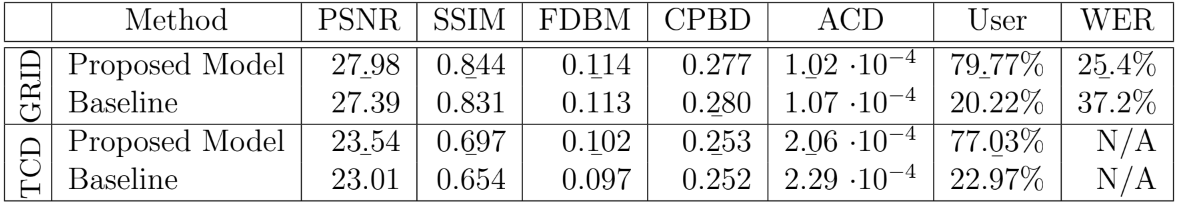
\includegraphics[width=15cm]{./content/images/vou2019_result.png}
    \caption{Kết quả của nghiên cứu End-to-End Speech-Driven Facial Animation with Temporal GANs}
    \label{fig:vou2019_result}
\end{figure}

Mô hình trong bài nghiên cứu đem lại tín hiệu khả quan cho việc tạo sinh ảnh khuôn mặt dựa trên tiếng nói. Phương pháp tạo sinh và các bộ phân biệt ảnh áp dụng phương pháp CGANs một cách hiệu quả nhằm mục đích tạo sự chân thật cho chuỗi ảnh. Một số kết quả được công bố bởi tác giả bài nghiên cứu cho thấy ảnh được tạo sinh có chất lượng tốt, không bị hiện tượng nhảy hình, độ ổn định khung hình tốt, có thể đánh lừa người xem qua phép thử Turing. Theo đó, có tới 79.77\% chuỗi hình ảnh bị đánh nhãn sai (được tạo sinh hay video thật) trên tập dữ liệu GRID và 77.03\% trên tập dữ liệu TCD. Tuy nhiên, một số hạn chế vẫn chưa được giải quyết. Thứ nhất, ngoài vùng miệng, bộ tạo sinh hình ảnh và các bộ phân biệt vẫn chưa chú trọng đến các phần khác trong khuôn mặt nhất là phần nửa trên. Điều này làm cho hình ảnh được tạo sinh thiếu tự nhiên so với video thực tế. Thứ hai, khuôn mặt vẫn chưa thể hiện được cảm xúc tương ứng với tiếng nói. Việc này cũng góp phần làm cho video được tạo sinh dễ bị nhận biết bởi người xem tinh ý. Thứ ba, chuyển động của đầu cũng không được thể hiện trong video làm cho video trở nên cứng nhắc và giả tạo nếu chiếu trong thời gian dài. Thứ tư, sự đồng bộ của tiếng nói và hình ảnh chưa được quan tâm và chưa có cơ chế đảm bảo hình ảnh được tạo sinh sẽ được căn giờ chuẩn xác với âm thanh.

%------------------------------------------------------------------------

\section{Bài nghiên cứu "Realistic Speech-Driven Facial Animation with GANs"\cite{vougioukas2020}}

Đây là bài nghiên cứu có cùng tác giả với bài nghiên cứu trong phần \ref{sec:vougioukas2019}. Với cùng mục tiêu và phương pháp tiếp cận tương đồng với nghiên cứu được công bố  năm 2019, Vougioukas đã có một số cập nhật, bổ sung và đánh giá cho mô hình được xây dựng. Trong nghiên cứu này, Vougioukas đã thêm vào mạng trước đó một bộ phân biệt mới, bộ phân biệt này giúp đảm bảo sự đồng bộ giữa hình ảnh được tạo sinh và tiếng nói tương ứng. Kiến trúc được cập nhật mới thể hiện ở hình \ref{fig:vou2020_model}.

\begin{figure}[H]
    \centering
    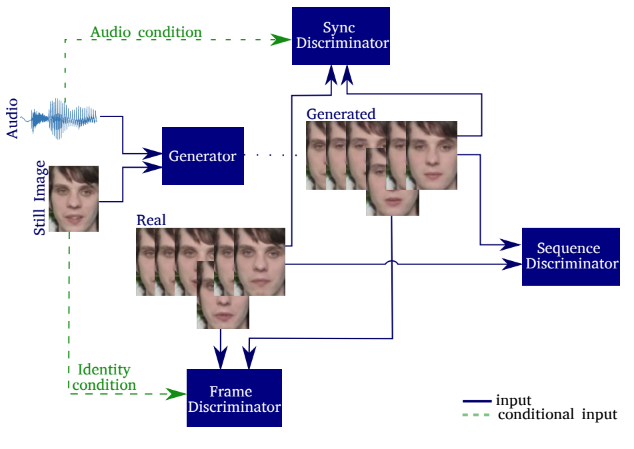
\includegraphics[width=9cm]{./content/images/vou2020_model.png}
    \caption{Kiến trúc mạng được cập nhật trong nghiên cứu mới của Vougioukas}
    \label{fig:vou2020_model}
\end{figure}

Bộ phân biệt tính đồng bộ Sync Discriminator được thể hiện trong hình \ref{fig:vou2020_sync_dis}. Bộ phân biệt này nhận vào một chuỗi hình ảnh nửa dưới (phần ảnh chứa vùng miệng) của mặt người đang nói. Chuỗi hình ảnh này có thể được tạo sinh bởi mạng sinh ảnh Generator hoặc là chuỗi ảnh thật được trích xuất từ video. Đồng thời, mạng cũng nhận vào đoạn tiếng nói tương ứng với chuỗi hình ảnh trên. Dữ liệu đưa vào mạng được thể hiện trong hình \ref{fig:vou2020_sync_input}. Chuỗi hình ảnh được đưa vào gồm 5 ảnh gồm $96 \times 64$ điểm ảnh tạo thành một tensor ba chiều. Tensor này được biến biến đổi thành ma trận hai chiều nhờ một lớp 3D Convolution. Sau đó, ma trận này tiếp tục được trích xuất đặc trưng nhờ ba lớp 2D Convolution và ở cuối là một lớp tuyến tính. Đặc trưng ảnh sau cùng được trích xuất là một vector 256 chiều. Đối với tiếng nói, quy trình trích xuất đặc trưng cũng được áp dụng trên vector âm thanh 8000 chiều. Bộ trích xuất đặc trưng âm thanh được sử dụng bao gồm 5 lớp 1D Convolution và cuối cùng là một lớp tuyến tính. Đặc trưng âm thanh cũng được trích xuất thành một vector 256 chiều. Khoảng cách Euclide giữa hai vector được tính toán theo công thức $d = \Vert \textrm{e}_{\textrm{sm}} - \textrm{e}_{\textrm{a}} \Vert$, với $\textrm{e}_{\textrm{sm}}$ và $\textrm{e}_{\textrm{a}}$ lần lượt là vector đặc trưng chuỗi hình ảnh và vector đặc trưng tiếng nói. Khoảng cách $d$ sau đó được đưa vào một lớp Perceptron để đưa ra sự đo đạc về độ phù hợp giữa chuỗi hình ảnh vùng miệng và âm thanh được đưa vào dưới dạng xác suất.

\begin{figure}[H]
    \centering
    \begin{minipage}{0.48\textwidth}
        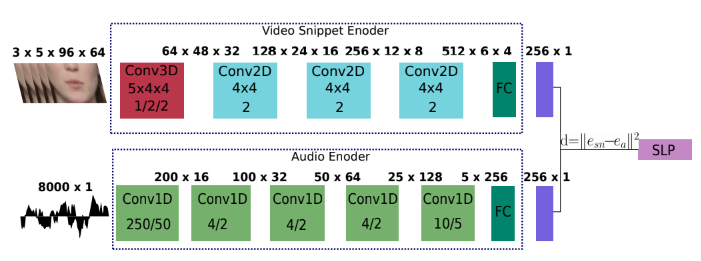
\includegraphics[width=7cm]{./content/images/vou2020_sync_dis.png}
        \caption{Kiến trúc bộ phân biệt đồng bộ Sync Discriminator}
        \label{fig:vou2020_sync_dis}
    \end{minipage}\hfill
    \begin{minipage}{0.48\textwidth}
        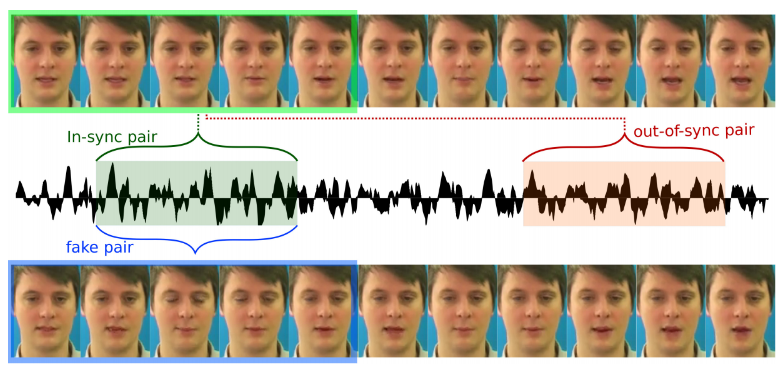
\includegraphics[width=7cm]{./content/images/vou2020_sync_input.png}
        \caption{Miêu tả dữ liệu được đưa vào mạng phân biệt đồng bộ}
        \label{fig:vou2020_sync_input}
    \end{minipage}
\end{figure}

Để có khả năng phân biệt tốt nhất, cặp hình ảnh - tiếng nói được đưa vào mạng được chọn lựa theo ba hoàn cảnh (xem hình \ref{fig:vou2020_sync_input}). Cặp đồng bộ đúng (in-sync pair), là cặp hình ảnh - tiếng nói tương ứng với nhau trong video. Cặp không đồng bộ (out-of-sync pair) gồm hình ảnh được trích xuất từ video nhưng không phù hợp với tiếng nói. Cuối cùng là cặp giả mạo (fake pair) gồm hình ảnh được tạo sinh vào tiếng nói tương ứng tạo sinh ra nó. Nhờ ba cặp này, mạng sẽ học được cách phân biệt sự sai lệch hình ảnh - tiếng nói và đặc biệt là sự đồng bộ của khẩu hình miệng với tiếng nói được cải thiện đáng kể.

Hàm mất mát phân biệt $\mathcal{L}_{adv}$ của mạng cũng được cập nhật thêm hàm mất mát của bộ phân biệt đồng bộ. Qua đó:

\begin{equation}
    \mathcal{L}_{adv} = \lambda_{img}\mathcal{L}^{img}_{adv} + \lambda_{adv}\mathcal{L}^{seq}_{adv} + \lambda_{seq}\mathcal{L}^{seq}_{adv}
    \label{eqn:vou2020_adv_loss}
\end{equation}

Với:
\begin{subequations}
    \begin{equation}
        \mathcal{L}^{img}_{adv} = \mathrm{E}_{x\sim P_d}[logD_{img}(S(x),x_1)] + \mathrm{E}_{z\sim P_z}[log(1 - D_{img}(S(G(z)), x_1))]
        \label{eqn:vou2020_img_loss}
    \end{equation}
    
    \begin{equation}
        \begin{split}
        \mathcal{L}^{seq}_{adv} = &\mathrm{E}_{x\sim P_d}[logD_{sync}(p_{in})] + \frac{1}{2}\mathrm{E}_{x\sim P_d}[log(1 - D_{sync}(p_{out}))] + \\
        &\frac{1}{2}\mathrm{E}_{z\sim P_z}[log(1 - D_{sync}(S_{snip}(p_{\textit{f}})))]
        \end{split}
        \label{eqn:vou2020_sync_loss}
    \end{equation}
    
    \begin{equation}
        \mathcal{L}^{seq}_{adv} = \mathrm{E}_{x\sim P_d}[logD_{seq}(x,a)] + \mathrm{E}_{z\sim P_z}[log(1 - D_{seq}(G(z), a))]
        \label{eqn:vou2020_seq_loss}
    \end{equation}
\end{subequations}

Bài nghiên cứu này đã mang lại cải tiến đáng kể cho nghiên cứu trước đó của tác giả. Đặc biệt là cải tiến về mặt đồng bộ về hình ảnh và âm thanh. Điều này giúp cho khẩu hình miệng trở nên chân thật và khớp với hình ảnh được thể hiện qua việc giảm đáng kể độ đo WER (đo độ sai sót của mô hình LipNet - mô hình đọc hình ảnh để đoán từ đang được nói). Các cử động nhỏ trên gương mặt cũng được tái hiện một cách tự nhiên hơn. Bảng sau là kết quả được khảo sát và đo đạc bởi tác giả Vougioukas trên bốn tập dữ liệu GRID, TCD, CREMA và LRW được xử lý bởi bốn mô hình khác nhau:

\begin{figure}[H]
    \centering
    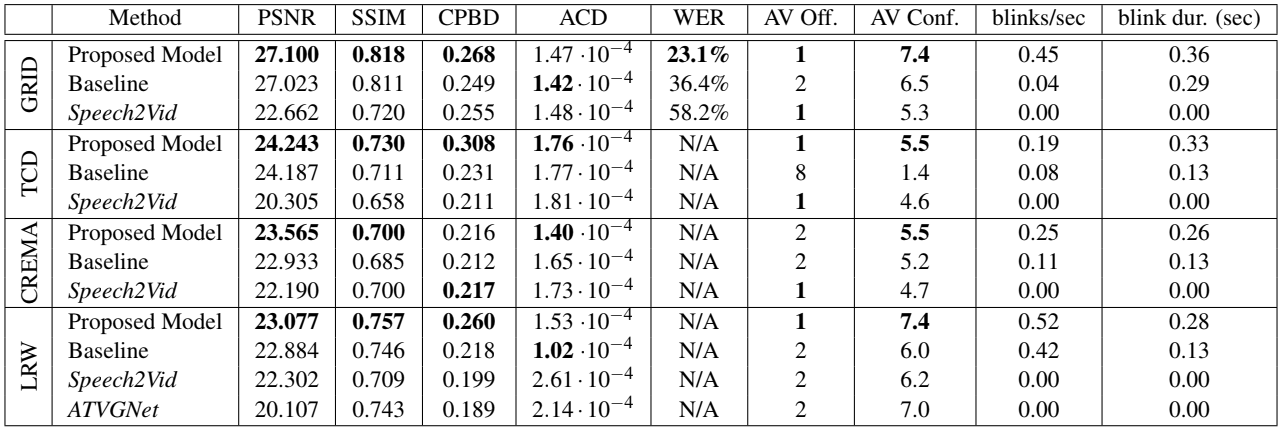
\includegraphics[width=15cm]{./content/images/vou2020_result.png}
    \caption{Kết quả đo đạc của tác giả}
    \label{fig:vou2020_result}
\end{figure}

Qua bảng này, ta thấy độ đo WER là rất thấp so với các mô hình khác nhờ vào sự phù hợp của vùng miệng so với ngữ điệu và nội dung tiếng nói. Các độ đo cơ bản khác như PSNR, SSIM và CPBD cũng được cải thiện so với các mô hình khác. Độ lệch về hình ảnh - âm thanh (AV Off.) cũng rất nhỏ (1). Điểm tự tin về sự đồng bộ giữa hình ảnh - âm thanh (AV Confident) được cải thiện rõ rệt và là bước tiến lớn so với các mô hình khác. Chuyển động của mắt cũng được đo đạc về số lần nháy mắt mỗi giây và thời lượng của một cái nháy mắt. Chuyển động của mắt trong video cũng là rất tự nhiên và đúng với chuyển động nháy mắt của người về tần số và thời lượng.
Ngoài các ưu điểm kể trên, một số yếu điểm từ nghiên cứu cũ được nêu ở phần \ref{sec:vougioukas2019} vẫn chưa được giải quyết. Đó là các yếu điểm về mặt biểu cảm trên gương mặt và chưa thể hiện được chuyển động của đầu. Ngoài ra, nghiên cứu cũng chưa chú trọng việc tái hiện lại môi trường xung quanh trong video. Qua kiểm nghiệm thực tế, mô hình còn cho thấy một yếu điểm khác khi không giữ được đặc điểm gương mặt của người mẫu nếu hình ảnh người này không tồn tại trong tập dữ liệu huấn luyện. Tác giả đã chạy thử mô hình với hình ảnh người châu Á (mô hình được huấn luyện với bộ dữ liệu mặt người phương Tây), mô hình cho ra mặt người đang nói với đặc trưng gương mặt không còn giống với người châu Á và không giữ được các đường nét đặc trưng của gương mặt người mẫu.

%------------------------------------------------------------------------

\section{Bài nghiên cứu "Hierarchical Cross-Modal Talking Face Generation with Dynamic Pixel-Wise Loss"\cite{chen2019}}

Nghiên cứu của Lele Chen vào năm 2019 có cùng mục tiêu với các nghiên cứu của Vougioukas, đó là tạo sinh chuỗi hình ảnh mặt người phù hợp với tiếng nói với đầu vào là một ảnh tĩnh của người mẫu và một đoạn âm thanh chứa tiếng nói. Trong nghiên cứu này, Chen đã đề xuất phương pháp mạng GANs nối tiếp để thiết kế bộ tạo sinh và phân biệt ảnh nhằm mục đích loại bỏ các đặc trưng không liên quan nhau trong miền đặc trưng ẩn. Nghiên cứu cũng làm rõ tầm quan trọng của việc sử dụng các đặc trưng trung gian thay vì sử dụng trực tiếp các đặc trưng được tổng hợp từ đầu vào. Nghiên cứu cũng sử dụng cơ chế chú ý (attenttion) để đánh dấu các điểm có sự biến đổi mạnh trên khuôn mặt dựa trên các đặc trưng ẩn được trích xuất. Cơ chế mạng phân biệt hồi quy cũng được tác giả giới thiệu nhằm mục đích giúp cho mạng phân biệt trích xuất đặc trưng có quan tâm đến thời gian để có thể dễ dàng phân biệt giữa video thật và video được tạo sinh. Qua đó, Lele Chen đã đóng góp thêm nhiều phương pháp mới để tạo sinh khuôn mặt và hạn chế sự giả tạo trong ảnh đầu ra. 

\begin{figure}[H]
    \centering
    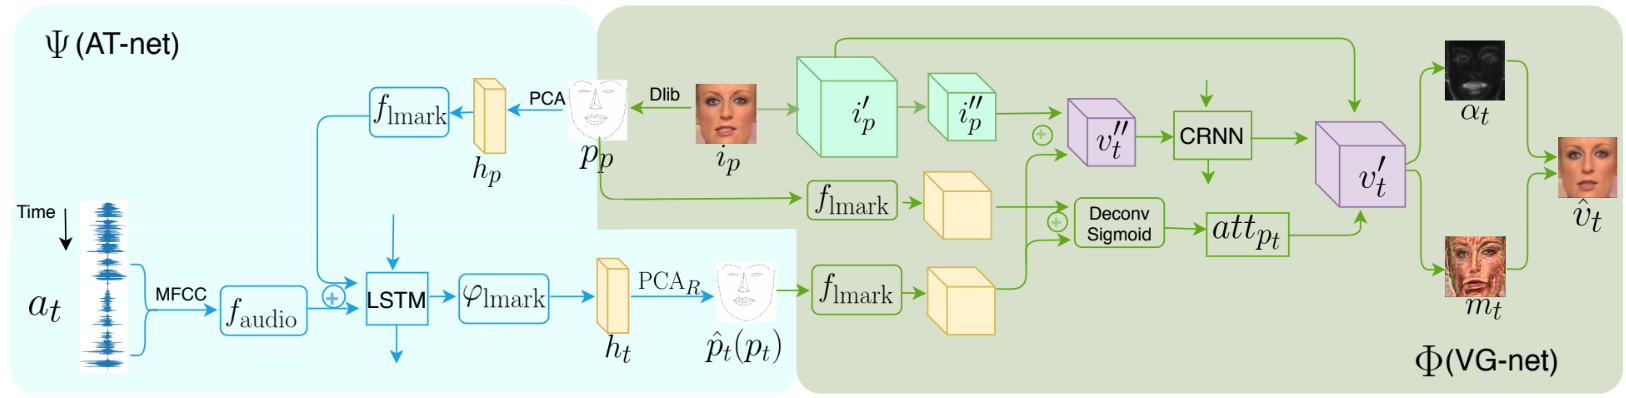
\includegraphics[width=15cm]{./content/images/chen2019_model.png}
    \caption{Mô hình được đề xuất bới nghiên cứu Hierarchical Cross-Modal Talking Face Generation with Dynamic Pixel-Wise Loss}
    \label{fig:chen2019_model}
\end{figure}

Hình \ref{fig:chen2019_model} thể hiện kiến trúc chung của mô hình được đề xuất. Mô hình tạo sinh ảnh được chia thành hai phần chính: phần trích xuất đặc trưng âm thanh $\Psi$ (AT-net) và phần tạo sinh hình ảnh $\Phi$ (VG-net). Với việc chia cấu trúc tổng quan thành hai phần nối tiếp nhau, ta có công thức thể hiện cơ chế tính toán của mạng:

\begin{subequations}
    \begin{equation}
        \hat{p}_{1:T} = \Psi(a_{1:T}, p_p)
    \end{equation}
    \begin{equation}
        \hat{v}_{1:T} = \Phi(\hat{p}_{1:T}, i_p, p_p)
    \end{equation}
\end{subequations}

Với $a_{1:T}$ là tín hiệu tiếng nói, $i_p$ là hình khuôn mặt của người mẫu, $p_p$ là các cột mốc (landmark) được trích xuất trên hình $i_p$, mô hình sẽ tạo sinh ra các cột mốc tương ứng với âm thanh $\hat{p}_{1:T}$ và dựa trên các cột mốc đó để dựng lại hình ảnh khuôn mặt $\hat{v}_{1:T}$.

Đầu tiên, các cột mốc trong ảnh mẫu $i_p$ được trích xuất bằng thư viện Dlib dùng phương pháp HOG. Bộ $\Psi$ (AT-net) nhận vào cột mốc $p_p$, sau đó dùng phương pháp PCA để thu giảm số chiều của vector cột mốc thành một vector đặc trưng $h_p$. Với việc sử dụng PCA, ngoài tác dụng giảm số chiều, tác giả còn có mục đích giảm nhiễu trên dữ liệu, từ đó giúp loại bỏ các chuyển động không mong muốn và các chuyển động không liên quan đến tiếng nói của các cột mốc như sự di chuyển của đầu, sự chuyển động của máy thu hình. Một bộ encoder $f_{lmark}$ được sử dụng để trích xuất đặc trưng cho các cột mốc. Đồng thời, tín hiệu âm thanh $a_{1:T}$ cũng được chuyển sang miền tần số  nhờ MFCC và được trích xuất đặc trưng nhờ bộ encoder $f_{audio}$. Vector đặc trưng cột mốc sẽ được ghép nối với tất cả vector đặc trưng tiếng nói theo kênh và đưa vào một bộ LSTM. Bộ LSTM hoạt động theo chiến thuật teacher forcing để sinh ra chuỗi các trạng thái ẩn (hidden state). Chuỗi trạng thái này được sử dụng như đặc trưng đầu ra và được đưa vào bộ decoder $\phi_{lmark}$ để tạo ra vector đặc trưng $h_t$ thể hiện các đặc trưng cột mốc của gương mặt sẽ được tạo sinh. Để tạo sinh ra cột mốc đó, ta dùng phép PCA ngược $PCA_R$ để đưa $h_t$ về chiều không gian của ma trận cột mốc và từ đó sinh ra cột mốc được dự đoán $\hat{p}_t$. Với việc sử dụng đặc trưng âm thanh và cột mốc để tạo sinh cột mốc mới theo thời gian thay vì trực tiếp sử dụng hình ảnh, nghiên cứu đã chỉ ra cách để tách biệt mục tiêu tái tạo chính xác khẩu hình miệng với các mục tiêu khác. Nhờ đó khẩu hình miệng được tái tạo chính xác hơn so với các nghiên cứu trước đó.

\begin{subequations}
    \begin{equation}
        v''_t = f_{img}(i_p) \oplus (f_{lmark}(\hat{p}_t) - f_{lmark}(p_p))
        \label{eqn:chen2019_vgnet_1}
    \end{equation}
    \begin{equation}
        att_{p_t} = \sigma(f_{lmark}(p_t) \oplus f_{lmark}(p_p))
        \label{eqn:chen2019_vgnet_2}
    \end{equation}
    \begin{equation}
        v'_t = (CRNN(v''_t)) \odot att_{p_t} + i'_p \oplus (1 - att_{p_t})
        \label{eqn:chen2019_vgnet_3}
    \end{equation}
\end{subequations}

Mạng tạo sinh ảnh $\Phi$ (VG-net) được xây dựng với mục tiêu duy trì các đặc tính trên khuôn mặt mẫu được cho ban đầu và tạo sự ổn định, liền lạc cho sự chuyển động giữa các khung hình. Hình ảnh mẫu $i_p$ được trích đặc trưng bằng một Convolution encoder và tạo ra tensor $i''_p$. Đồng thời, cột mốc $p_p$ và $\hat(p)_t$ cũng được trích đặc trưng nhờ các bộ encoder $f_{lmark}$. Tác giả giả định rằng sự sai lệch giữa vector cột mốc được tạo sinh $\hat{p_t}$ và cột mốc trong ảnh mẫu $p_p$ sẽ tương ứng với sự sai lệch trong hình ảnh mặt người được tạo sinh và ảnh mẫu. Vì vậy, đặc trưng sai khác này được kết hợp với đặc trưng ảnh mẫu bằng cách nối tiếp theo kênh để tạo ra đặc trưng ảnh mới (công thức \ref{eqn:chen2019_vgnet_1}). Cũng với việc kết hợp đặc trưng cột mốc ảnh mẫu và cột mốc ảnh được tạo sinh, ta sẽ tìm được các vùng trên gương mặt có sự thay đổi lớn bằng các chuyển động của các cột mốc tương ứng nhau. Từ đó, ta có thể tính được ma trận chú ý (attention map) để đánh dấu các vùng có sự thay đổi lớn trên ảnh (công thức \ref{eqn:chen2019_vgnet_2}). Khối CRNN là một khối đạng encoder - decoder, chứa trong nó là các khối Convolution - RNN, các khối Residual và các lớp Deconvolution. Đặc trưng $v''_t$ theo thời gian được đưa qua khối CRNN để encode và decode nó trở lại, kết hợp với $att_{p_t}$ và $i'_p$ để tạo thành tensor đặc trưng $v't$ (công thức \ref{eqn:chen2019_vgnet_3}). Việc đưa $v''_t$ qua CRNN là để liên kết các chuyển động theo thời gian và tạo sinh đặc trưng có tính liên kết về mặt thời gian. Do mức độ ảnh hưởng của tiếng nói đối với các cột mốc trên ảnh là khác nhau, ma trận $att_{p_t}$ được nhân vào đặc trưng ngõ ra của CRNN để chọn lấy các cột mốc bị ảnh hưởng nhiều bởi tiếng nói, các cột mốc còn lại được lấy từ đặc trưng ảnh mẫu $i'_p$. Sau cùng, đặc trưng tổng hợp $v'_t$ sẽ được dùng để sinh ra một ma trận chú ý $\alpha_t$ và ảnh mô tả chuyển động $m_t$. $\alpha_t$ được sinh ra nhờ việc cho $v'_t$ đi qua một lớp Convolution và hàm kích hoạt Sigmoid, trong khi $m_t$ được sinh ra nhờ cho $v'_t$ đi qua một lớp Convolution khác với hàm kích hoạt $tanh$. Trong khi $\alpha_t$ có khả năng đánh dấu các điểm ảnh có nhiều sự thay đổi trên ảnh được tạo sinh so với ảnh gốc bằng các giá trị xác suất cao, $m_t$ là một ảnh miêu tả chuyển động trên gương mặt tương ứng với âm thanh tại thời điểm $t$. Để có kết quả tạo sinh hoàn hảo, ổn định và giống với người mẫu nhất, ta sẽ kết hợp ảnh $m_t$ với ảnh $i_p$ ban đầu với tỉ lệ nhìn thấy của mỗi điểm ảnh trên mỗi ảnh được thể hiện qua ma trận chú ý $\alpha_t$. Ảnh đầu ra cuối cùng $\hat{v}_t$ được tạo sinh như sau: 

\begin{equation}
    \hat{v}_t = \alpha_t \odot m_t + (1 - \alpha_t) \odot i_p
\end{equation}

\begin{equation}
    \mathcal{L}_{pix} = \sum^{T}_{t=1} \Vert (v_t - \hat{v}_t) \odot (\overline{\alpha}_t + \beta) \Vert_1
    \label{eqn:chen2019_pix_loss}
\end{equation}

Hàm mất mát theo điểm ảnh được sử dụng trong công thức (\ref{eqn:chen2019_pix_loss}) cho thấy nó chỉ quan tâm nhiều tới các điểm ảnh có trọng số cao trong ma trận $\alpha_t$. $\beta$ là một hằng số, được cộng thêm vào hàm mất mát nhằm mục đích đảm bảo điểm ảnh nào cũng có đóng góp vào hàm mất mát, tránh hiện tượng $\alpha_t$ về 0.

\begin{figure}[H]
    \centering
    \begin{minipage}{0.48\textwidth}
        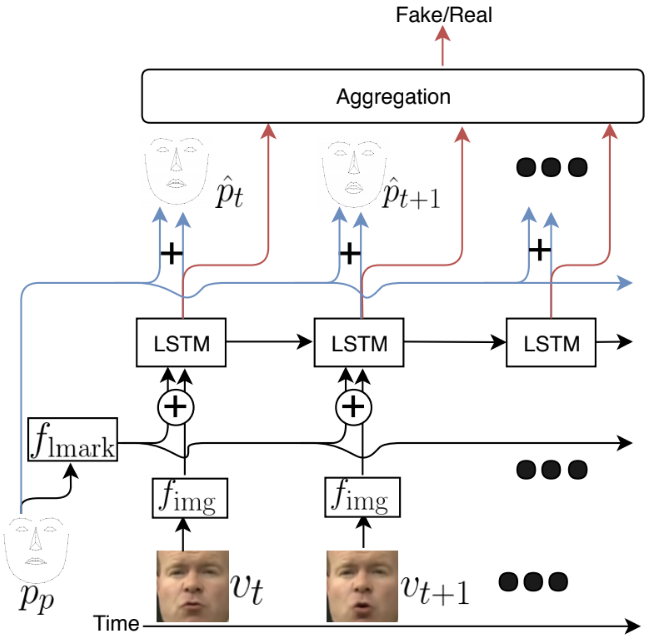
\includegraphics[width=7cm]{./content/images/chen2019_dis.png}
        \caption{Kiến trúc bộ phân biệt}
        \label{fig:chen2019_dis}
    \end{minipage}\hfill
    \begin{minipage}{0.48\textwidth}
        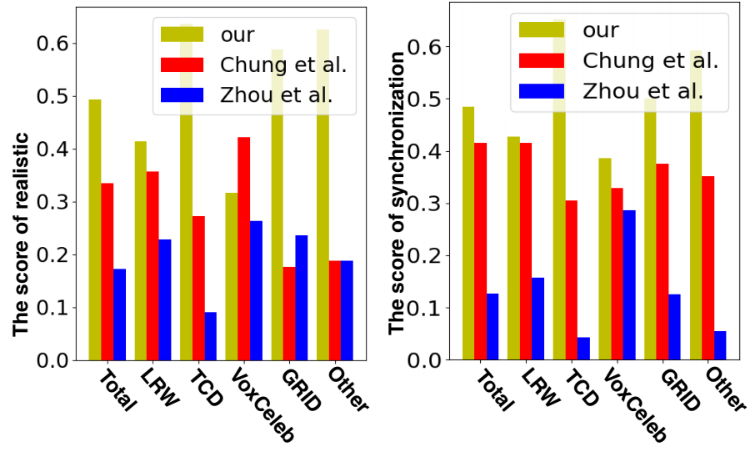
\includegraphics[width=7cm]{./content/images/chen2019_score.png}
        \caption{So sánh kết quả các mô hình}
        \label{fig:chen2019_score}
    \end{minipage}
\end{figure}

Bộ phân biệt được thiết kế để phân biệt chuỗi hình ảnh được đưa vào $v_t$ là chuỗi hình ảnh thật từ video hay chuỗi hình ảnh được tạo sinh. Bộ phân biệt này có chức năng phân biệt tổng quát trên toàn bộ chuỗi ảnh và cho từng ảnh một trong chuỗi. Công thức của bộ phân biệt được thể hiện như sau:

\begin{subequations}
    \begin{equation}
        \begin{split}
            \hat{p}_t &= D_p(p_p, v_t) \\
            &= p_p + LSTM(f_{lmark}(p_p) \oplus f_{img}(v_t))
        \end{split}
        \label{eqn:chen2019_dis_dp}
    \end{equation}
    \begin{equation}
        \begin{split}
            s &= D_s(p_p, v_{1:T}) \\
            &= \sigma(\frac{1}{T} \sum^T_{t=1} LSTM(f_{lmark}(p_p) \oplus f_{img}(v_t)))
        \end{split}
        \label{eqn:chen2019_dis_ds}
    \end{equation}
    \begin{equation}
        \begin{split}
        \mathcal{L}_{gan} = &\mathbb{E}_{p_p,v_{1:T}}[logD_s(p_p,v_{1:T})]+\\
        &\mathbb{E}_{p_p,v_{1:T},i_p}[log(1-D_s(p_p,G(p_p,p_{1:T},i_p)))]+\\
        &||(D_p(p_p,G(p_p,p_{1:T},i_p))-p_{1:T}) \odot M_p||^2_2+\\
        &||(D_p(p_p,v_{1:T})-p_{1:T}) \odot M_p||^2_2
        \end{split}
        \label{eqn:chen2019_dis_gan}
    \end{equation}
\end{subequations}

Kết quả đo đạc của tác giả được thể hiện ở bảng sau:
\begin{figure}[H]
    \centering
    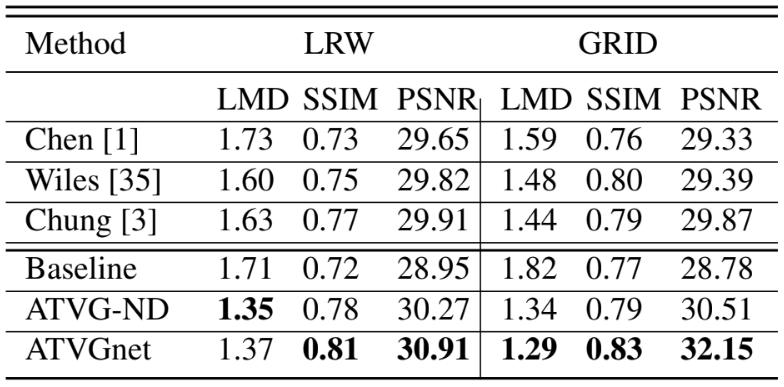
\includegraphics[width=10cm]{./content/images/chen2019_result.png}
    \caption{}
    \label{fig:chen2019_result}
\end{figure}

Qua bảng này, ta thấy nghiên cứu của tác giả đã có sự cải tiến khi làm giàu thêm tri thức của mạng về bài toán với việc thay thế đặc trưng âm thanh bằng các cột mốc gương mặt. Và với bộ phân biệt, không chỉ học được cách nhận biết ảnh thật và giả như các nghiên cứu trước mà còn học được cách tạo dựng lại các cột mốc trên gương mặt ban đầu. Nhờ đó mạng phân biệt có nhiều tri thức hơn để giúp điều chỉnh mạng tạo sinh nhằm tạo ra những chuyển động chân thật cho gương mặt. Thiết kế của mạng không nhằm mục đích tạo sinh hoàn toàn hình ảnh khuôn mặt, mà thay vào đó, mạng chỉ cố gắng mô tả những thay đổi phải thực hiện trên hình ảnh mẫu để tạo ra ảnh tạo sinh. Điều này làm cho hình ảnh tạo sinh có chất lượng tốt và giữ được đặc trưng riêng của người mẫu.
